\documentclass{llncs}

\usepackage[utf8]{inputenc}
\usepackage[T1]{fontenc}
\usepackage[english]{babel}
\usepackage{booktabs}
\usepackage{array}
\usepackage{amsmath}
\usepackage{amssymb}
\usepackage{tikz}
\usetikzlibrary{positioning,shapes,arrows,calc}
\usepackage{listings}
\usepackage{xcolor}
\usepackage[hidelinks]{hyperref}
\usepackage{float}
\usepackage{enumitem}
\usepackage{multirow}
\usepackage{pgfplots}
\pgfplotsset{compat=1.18}
\usepackage{caption}
\usepackage{graphicx}

\definecolor{codebg}{RGB}{248,248,248}
\definecolor{codeframe}{RGB}{200,200,200}
\definecolor{kwcolor}{RGB}{0,0,180}
\definecolor{cmtcolor}{RGB}{100,100,100}
\definecolor{strcolor}{RGB}{160,0,0}

\lstdefinestyle{python}{
  language=Python,
  basicstyle=\ttfamily\scriptsize,
  keywordstyle=\color{kwcolor}\bfseries,
  commentstyle=\color{cmtcolor}\itshape,
  stringstyle=\color{strcolor},
  breaklines=true,
  frame=single,
  rulecolor=\color{codeframe},
  backgroundcolor=\color{codebg},
  xleftmargin=0.5em,
  aboveskip=0.4em,
  belowskip=0.4em,
}

\lstdefinestyle{prolog}{
  language=Prolog,
  basicstyle=\ttfamily\scriptsize,
  keywordstyle=\color{kwcolor}\bfseries,
  commentstyle=\color{cmtcolor}\itshape,
  stringstyle=\color{strcolor},
  breaklines=true,
  frame=single,
  rulecolor=\color{codeframe},
  backgroundcolor=\color{codebg},
  xleftmargin=0.5em,
  aboveskip=0.4em,
  belowskip=0.4em,
}

% ─────────────────────────────────────────────────────────────────────────────
\begin{document}

\title{Multi-Tenant Mobile Antenna Placement Optimization}
\subtitle{A Comparative Study of OR-Tools CP-SAT and SICStus CLP(FD)}

\author{Martim Pinheiro \and Adam Oprchal}

\institute{
  Faculdade de Engenharia da Universidade do Porto, Porto, Portugal \\
  \email{\{up20509641, up202512712\}@fe.up.pt}
}

\maketitle

% =============================================================================
\begin{abstract}
We formulate Multi-Tenant Mobile Antenna Placement as a Constraint Satisfaction
and Optimisation Problem (CSOP) over Boolean finite domains and implement it in
two constraint programming solvers: Google OR-Tools CP-SAT and SICStus Prolog
CLP(FD). Given a grid map with heterogeneous terrain, the model places cell
towers and assigns antennas from four telecom providers with distinct Manhattan
coverage radii to minimise total infrastructure cost, comprising tower
construction, antenna slot fees, and soft-constraint uncoverage penalties.
Both implementations share the same mathematical model and a common data
pipeline. Benchmarks across grid sizes from $4{\times}4$ to $64{\times}64$
confirm model equivalence and reveal a large scalability gap: OR-Tools solves
instances up to $16{\times}16$ within 60 seconds, while SICStus times out
beyond $5{\times}5$. The root causes --- CDCL clause learning, LP-based lower
bounds, and internal symmetry detection in CP-SAT versus pure arc-consistency
propagation in CLP(FD) --- are analysed in depth. Post-presentation
improvements, including the first-fail (\texttt{ff}) labelling heuristic and
extended OR-Tools benchmarks, are evaluated and discussed.
\end{abstract}

\keywords{Constraint Programming \and Antenna Placement \and OR-Tools CP-SAT
\and SICStus CLP(FD) \and Combinatorial Optimisation \and Network Planning}

% =============================================================================
\section{Introduction}
\label{sec:intro}
% =============================================================================

Mobile network planning is a large-scale combinatorial optimisation problem:
operators must decide where to build physical infrastructure and which radio
services to assign to each site, subject to technical, financial, and regulatory
constraints. In a \emph{multi-tenant} setting, multiple operators co-locate
equipment on shared cell towers, reducing capital expenditure while increasing
site density.

This work addresses a representative instance: given a grid map with four
terrain types, place cell towers and assign antennas from four providers to
minimise total infrastructure cost. Coverage is a \emph{soft constraint}
modelled via a financial penalty, allowing the solver to trade tower
construction against unserved cells. Two contrasting Constraint Programming (CP)
platforms are implemented and compared:
\begin{itemize}
  \item \textbf{Google OR-Tools CP-SAT}~\cite{ortools}: a hybrid solver
        combining Conflict-Driven Clause Learning (CDCL) with LP relaxations.
  \item \textbf{SICStus Prolog CLP(FD)}~\cite{sicstus}: a classical
        finite-domain solver based on arc-consistency propagation and
        branch-and-bound search.
\end{itemize}

Implementing the same model in both solvers allows a direct empirical comparison
of two CP paradigms and provides concrete evidence of how solver architecture
affects scalability on a realistic problem.

% =============================================================================
\section{Problem Description}
\label{sec:problem}
% =============================================================================

\subsection{Grid and Terrain}

The search space is an $R{\times}C$ grid of cells, each with one of four
terrain types that determine tower buildability and cost
(Table~\ref{tab:terrain}). Terrain is generated randomly with fixed
proportions: 12\% mountains (banned), 20\% forest, 15\% building, remainder
plains.

\begin{table}[H]
\centering
\caption{Terrain types and tower construction costs.}
\label{tab:terrain}
\begin{tabular}{llrc}
\toprule
\textbf{Terrain} & \textbf{Symbol} & \textbf{Tower cost (€)} & \textbf{Buildable?} \\
\midrule
Plains   & \texttt{.} & 1\,000 & Yes \\
Forest   & \texttt{F} & 1\,500 & Yes \\
Building & \texttt{B} & 2\,500 & Yes \\
Mountain & \texttt{M} & ---    & No  \\
\bottomrule
\end{tabular}
\end{table}

\subsection{Telecom Providers and Coverage}

Four providers (P0--P3) operate on different frequency bands with different
Manhattan-radius coverage patterns (Table~\ref{tab:providers}). An antenna at
cell $i$ covers all non-banned cells within Manhattan distance $r_k$.

\begin{table}[H]
\centering
\caption{Provider frequency bands and coverage radii.}
\label{tab:providers}
\begin{tabular}{clcc}
\toprule
\textbf{Provider} & \textbf{Band} & \textbf{Radius $r_k$} & \textbf{Technology} \\
\midrule
P0 & High-band / 5G mmWave & 0 & Own cell only \\
P1 & Mid-band / 4G--5G     & 1 & Adjacent cells \\
P2 & Mid-band / 4G--5G     & 1 & Adjacent cells \\
P3 & Low-band / Macro LTE  & 2 & Wide area \\
\bottomrule
\end{tabular}
\end{table}

P1 and P2 share radius $r{=}1$, introducing solution symmetry: swapping their
placements yields an identical-cost solution. This doubles the effective search
space unless broken explicitly (Section~\ref{sec:sym}).

\subsection{Cost Structure}

Total cost has three additive components:
(1)~tower construction (€1\,000--€2\,500, terrain-dependent);
(2)~antenna slot fees (€100 per antenna);
(3)~uncoverage penalties (€800 per uncovered provider--cell pair).
The penalty mechanism transforms coverage into a soft constraint: covering a
remote cell is skipped when its cost exceeds the penalty savings.

% =============================================================================
\section{Formal Model}
\label{sec:model}
% =============================================================================

Let $N{=}R{\times}C$, $K{=}4$, $\mathcal{B}$ the banned cells, and
$\mathcal{C}{=}[0,N){\setminus}\mathcal{B}$ the coverable cells.

\smallskip\noindent\textbf{Decision variables:}
\begin{align}
t_i &\in \{0,1\} \quad i \in [0,N) \notag\\
a_{k,i} &\in \{0,1\} \notag\\
s_{k,j} &\in \{0,1\} \quad j \in \mathcal{C} \notag
\end{align}

$t_i = 1$ means a physical tower is erected at cell $i$; $t_i = 0$ means the
cell is left empty. $a_{k,i} = 1$ means provider $k$ installs an antenna at
cell $i$. $s_{k,j} = 1$ means cell $j$ is \emph{not} covered by provider $k$,
activating the financial penalty for that pair. Total variables:
$N + KN + K|\mathcal{C}|$ (308 for a $6{\times}6$ grid).

\smallskip\noindent\textbf{Coverage sources:}
\[
\mathrm{cov}(k,j) = \{ i \in [0,N){\setminus}\mathcal{B} \mid \|i{-}j\|_1 \leq r_k \}
\]
$\mathrm{cov}(k,j)$ is the set of all non-banned cells from which an antenna of
provider $k$ would reach target cell $j$ within Manhattan distance $r_k$.
It is precomputed before the solver runs.

\smallskip\noindent\textbf{Constraints:}

\noindent\textbf{C1} \quad $t_i = 0 \;\forall i \in \mathcal{B}$

\noindent No tower may be built on a mountain cell. These cells are permanently
banned from the search space.

\smallskip
\noindent\textbf{C2} \quad $a_{k,i} \leq t_i \;\forall k,\forall i$

\noindent An antenna can only be installed where a physical tower already exists.
If no tower is built at cell $i$, all provider antenna variables for that cell
are forced to zero.

\smallskip
\noindent\textbf{C3} \quad $\displaystyle\sum_{k=0}^{K-1} a_{k,i} \leq 4 \;\forall i$

\noindent At most four providers may share a single tower. This is the
multi-tenancy capacity constraint; since $K = 4$ in this configuration, it
prevents a single tower from being over-committed if the number of providers
were extended in the future.

\smallskip
\noindent\textbf{C4} \quad
$\displaystyle\sum_{i \in \mathrm{cov}(k,j)} a_{k,i} + s_{k,j} \geq 1
\;\forall k,\forall j \in \mathcal{C}$

\noindent For every (provider, cell) pair, either at least one antenna within
coverage range is active, or the slack variable $s_{k,j}$ is set to 1. When the
slack is 1, the cell is left uncovered and the penalty is charged in the
objective. This is the \emph{reified} form of the coverage constraint: it
allows the solver to decide whether covering a particular cell is economically
worthwhile.

\smallskip\noindent\textbf{Objective:}
\[
\min Z = \underbrace{\sum_{i} c_i \, t_i}_{\text{tower construction}}
       + \underbrace{100 \sum_{k,i} a_{k,i}}_{\text{antenna slots}}
       + \underbrace{800 \sum_{k,j} s_{k,j}}_{\text{uncoverage penalties}}
\]

The first term accumulates the terrain-dependent tower construction cost
($c_i \in \{1000, 1500, 2500\}$) for every tower that is built. The second
term charges a flat €100 fee for each antenna slot used, regardless of provider
or terrain. The third term penalises every (provider, cell) pair that is left
without coverage. Because all three terms are linear combinations of Boolean
variables, the problem is also encodable as a Binary ILP.

% =============================================================================
\section{Implementation}
\label{sec:impl}
% =============================================================================

\subsection{System Architecture}

A single JSON file (\texttt{map\_data.json}) serves as the shared data source
for both solver pipelines (Fig.~\ref{fig:arch}). This guarantees both solvers
operate on exactly the same instance. A Python preprocessor
(\texttt{preprocessor.py}) translates the JSON into Prolog facts
(\texttt{map\_data.pl}) for the SICStus solver. A benchmark runner
(\texttt{benchmark.py}) orchestrates both solvers, collects timing and cost
data, and writes results to CSV.

\begin{figure}[H]
\centering
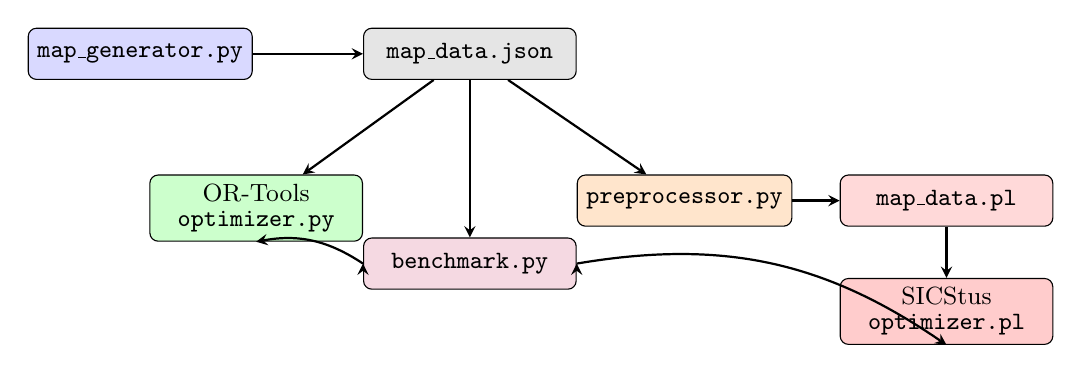
\begin{tikzpicture}[
  box/.style={draw, rounded corners=3pt, minimum width=2.7cm, minimum height=0.65cm,
              align=center, font=\small},
  arr/.style={->, thick, >=stealth}
]
  \node[box, fill=blue!15]   (gen)  {\texttt{map\_generator.py}};
  \node[box, fill=gray!20,   right=1.4cm of gen]  (json) {\texttt{map\_data.json}};
  \node[box, fill=green!20,  below left=1.2cm and 0.0cm of json]  (ort)  {OR-Tools\\[-2pt]\texttt{optimizer.py}};
  \node[box, fill=orange!20, below right=1.2cm and 0.0cm of json] (pre)  {\texttt{preprocessor.py}};
  \node[box, fill=red!15,    right=0.6cm of pre]  (pl)   {\texttt{map\_data.pl}};
  \node[box, fill=red!20,    below=0.65cm of pl]  (sic)  {SICStus\\[-2pt]\texttt{optimizer.pl}};
  \node[box, fill=purple!15, below=2.0cm of json] (bench){\texttt{benchmark.py}};
  \draw[arr] (gen)  -- (json);
  \draw[arr] (json) -- (ort);
  \draw[arr] (json) -- (pre);
  \draw[arr] (pre)  -- (pl);
  \draw[arr] (pl)   -- (sic);
  \draw[arr] (json) -- (bench);
  \draw[arr] (bench.west) edge[bend right=22] (ort.south);
  \draw[arr] (bench.east) edge[bend left=22]  (sic.south);
\end{tikzpicture}
\caption{System architecture: single JSON source feeds two independent solver
  pipelines and the shared benchmark runner.}
\label{fig:arch}
\end{figure}

\subsection{OR-Tools CP-SAT}

The OR-Tools implementation uses the \texttt{cp\_model} Python API.
All variables are \texttt{NewBoolVar} instances. Coverage sources are
precomputed once before model construction. The coverage-or-penalty constraint
C4 is posted as a single \texttt{model.Add(...)} call per (provider, cell) pair:

\begin{lstlisting}[style=python]
for (k, tgt), sources in coverage_sources.items():
    model.Add(sum(antennas[k][src] for src in sources)
              + slacks[k][tgt] >= 1)
\end{lstlisting}

The solver is configured with a wall-clock timeout and accepts both
\texttt{OPTIMAL} and \texttt{FEASIBLE} statuses.

\subsection{SICStus Prolog CLP(FD)}

The SICStus implementation uses \texttt{library(clpfd)}.
Variables are 0/1 domain lists: $T$ (towers), $P0$--$P3$ (antennas per
provider), $S0$--$S3$ (slacks per provider). Cost terms are built with
\texttt{scalar\_product/4} and summed via \texttt{\#=}. The coverage
constraint is expressed as:

\begin{lstlisting}[style=prolog]
extract_domain_vars(ValidSources, P_k, CoverageVars),
sum([SlackVar | CoverageVars], #>=, 1)
\end{lstlisting}

Optimisation uses branch-and-bound via \texttt{labeling/2}:

\begin{lstlisting}[style=prolog]
labeling([ff, minimize(GlobalCost)], AllVars)
\end{lstlisting}

The \texttt{ff} (first-fail) option branches on the variable with the smallest
remaining domain (see Section~\ref{sec:ff}).

% =============================================================================
\section{Experimental Results}
\label{sec:results}
% =============================================================================

\subsection{Setup}

All benchmarks use a 60-second timeout per solver, seed 42 for
reproducibility, and nine grid sizes from $4{\times}4$ to $64{\times}64$.
The benchmark runner invokes both solvers as independent subprocesses and
records wall-clock time, optimal cost, and coverage percentage.

\subsection{Results}

\begin{table}[H]
\centering
\caption{Benchmark results (60 s timeout, seed 42). T/O = timeout.}
\label{tab:benchmarks}
\begin{tabular}{lrrrrrr}
\toprule
\multirow{2}{*}{\textbf{Grid}} & \multirow{2}{*}{\textbf{Cells}}
  & \multicolumn{3}{c}{\textbf{OR-Tools CP-SAT}}
  & \multicolumn{2}{c}{\textbf{SICStus CLP(FD)}} \\
\cmidrule(lr){3-5}\cmidrule(lr){6-7}
& & Time (ms) & Cost (€) & Cov.\% & Time (ms) & Cost (€) \\
\midrule
$4{\times}4$   &    16 &      390 &   13\,600 & 82 &       371 &   13\,600 \\
$5{\times}5$   &    25 &      397 &   22\,500 & 84 &    14\,373 &   22\,500 \\
$6{\times}6$   &    36 &      418 &   31\,600 & 82 & \textsc{t/o} & --- \\
$7{\times}7$   &    49 &      461 &   42\,400 & 82 & \textsc{t/o} & --- \\
$8{\times}8$   &    64 &      495 &   55\,500 & 82 & \textsc{t/o} & --- \\
$12{\times}12$ &   144 &    1\,377 &  122\,600 & 82 & \textsc{t/o} & --- \\
$16{\times}16$ &   256 &   31\,112 &  218\,600 & 82 & \textsc{t/o} & --- \\
$32{\times}32$ & 1\,024 & \textsc{t/o} & --- & --- & \textsc{t/o} & --- \\
$64{\times}64$ & 4\,096 & \textsc{t/o} & --- & --- & \textsc{t/o} & --- \\
\bottomrule
\end{tabular}
\end{table}

\subsection{Model Correctness}

On all instances where both solvers complete ($4{\times}4$ and $5{\times}5$),
they produce \textbf{identical optimal costs}, confirming that both
implementations encode exactly the same CSOP. Additional multi-seed validation
(seeds 42, 123, 456 for $4{\times}4$--$5{\times}5$) yielded six matching
cost pairs across both solvers.

\subsection{Timing and Coverage}

Figure~\ref{fig:times} plots solve time on a log scale. The gap is already
visible at $5{\times}5$: OR-Tools solves in 397~ms; SICStus takes
14.4~s --- a \textbf{36× difference}. From $6{\times}6$ onward SICStus
consistently times out. OR-Tools scales to $16{\times}16$ (31~s) but also
times out at $32{\times}32$ (1\,024 cells), revealing its own ceiling.

Both solvers achieve \textbf{82--84\% coverage} on all completed instances.
The uncovered 16--18\% are economically rational: building a tower for those
cells costs more than the €800 penalty. Coverage is stable across all grid
sizes, confirming that the penalty formulation generalises uniformly.

\begin{figure}[H]
\centering
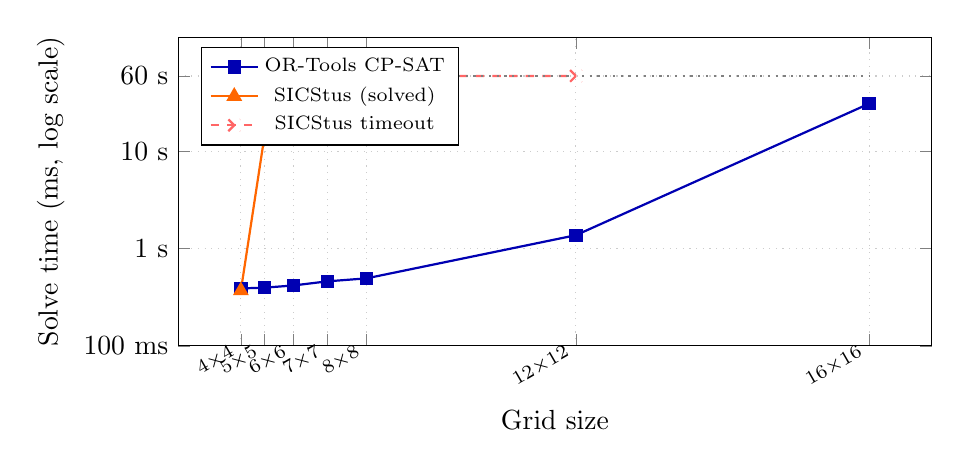
\begin{tikzpicture}
\begin{semilogyaxis}[
  width=0.92\textwidth, height=5.5cm,
  xlabel={Grid size}, ylabel={Solve time (ms, log scale)},
  xtick={16,25,36,49,64,144,256},
  xticklabels={$4{\times}4$,$5{\times}5$,$6{\times}6$,$7{\times}7$,
               $8{\times}8$,$12{\times}12$,$16{\times}16$},
  x tick label style={rotate=30, anchor=east, font=\scriptsize},
  legend pos=north west, legend style={font=\scriptsize},
  grid=major, grid style={dotted,gray!40},
  ymin=100, ymax=150000,
  ytick={100,1000,10000,60000},
  yticklabels={100 ms, 1 s, 10 s, 60 s},
]
\addplot[blue!70!black, thick, mark=square*, mark size=2pt] coordinates {
  (16,390)(25,397)(36,418)(49,461)(64,495)(144,1377)(256,31112)};
\addlegendentry{OR-Tools CP-SAT}
\addplot[orange!80!red, thick, mark=triangle*, mark size=2.5pt] coordinates {
  (16,371)(25,14373)};
\addlegendentry{SICStus (solved)}
\addplot[red!60, dashed, thick, mark=x, mark size=3pt] coordinates {
  (36,60063)(49,60062)(64,60062)(144,60035)};
\addlegendentry{SICStus timeout}
\draw[dotted,gray,thick](axis cs:16,60000)--(axis cs:256,60000);
\end{semilogyaxis}
\end{tikzpicture}
\caption{Solve-time comparison (log scale). SICStus data points for
  $6{\times}6$ and beyond all hit the 60-second ceiling.}
\label{fig:times}
\end{figure}

% =============================================================================
\section{Performance Analysis}
\label{sec:analysis}
% =============================================================================

Four compounding factors explain the scalability gap. These are not fundamental
CLP(FD) limitations --- they are configuration choices, each independently
addressable.

\subsection{Naive Variable Ordering}

Without heuristics, \texttt{labeling/2} assigns variables left-to-right:
towers first, then antennas, then slacks. The solver commits to a complete
tower layout before considering coverage, discovering conflicts late and
triggering expensive deep backtracking.

\subsection{Weak Lower Bounds}

SICStus branch-and-bound prunes branches only when constraint propagation can
prove cost exceeds the current best. These bounds are often loose. OR-Tools
CP-SAT solves an LP relaxation at each node, providing tight fractional lower
bounds that prune entire subtrees with a certificate of suboptimality.

\subsection{Arc Consistency vs.\ Clause Learning}

CLP(FD) uses arc-consistency propagation (AC-3/AC-4): sound and complete, but
memoryless --- backtracking discards all intermediate reasoning. OR-Tools
CP-SAT uses CDCL~\cite{sat}: on conflict, it analyses the implication graph,
derives a \emph{no-good clause}, and adds it permanently. Learned clauses
prune future branches that recreate the same conflict. CLP(FD) backtracks and
forgets; CP-SAT backtracks and \emph{learns}.

\subsection{Unhandled Solution Symmetry}
\label{sec:sym}

Providers P1 and P2 have identical radii ($r{=}1$). Swapping their placements
yields an equal-cost solution. Without a symmetry-breaking constraint, the
solver explores both symmetric halves, roughly doubling the search.
The fix is a single lexicographic ordering constraint:
$\texttt{lex\_chain([P1, P2])}$.
OR-Tools handles this internally; the SICStus model does not include it.

Table~\ref{tab:factors} summarises all four factors.

\begin{table}[H]
\centering
\caption{Performance gap factors and targeted remedies.}
\label{tab:factors}
\begin{tabular}{lll}
\toprule
\textbf{Factor} & \textbf{Impact} & \textbf{Remedy} \\
\midrule
Naive variable ordering & Late conflict detection    & \texttt{ff} heuristic \\
Weak lower bounds       & Poor subtree pruning       & LP relaxation \\
No clause learning      & Repeated identical conflicts & CDCL \\
Unhandled symmetry      & ${\approx}2{\times}$ search & \texttt{lex\_chain} \\
\bottomrule
\end{tabular}
\end{table}

% =============================================================================
\section{Implemented Improvements}
\label{sec:improvements}
% =============================================================================

\subsection{First-Fail Heuristic}
\label{sec:ff}

The \texttt{ff} variable ordering was added to the SICStus solver:

\begin{lstlisting}[style=prolog]
labeling([ff, minimize(GlobalCost)], AllVars)
\end{lstlisting}

Table~\ref{tab:ff} compares solve times before and after.

\begin{table}[H]
\centering
\caption{SICStus solve times with and without \texttt{ff} (seed 42).}
\label{tab:ff}
\begin{tabular}{lrrrr}
\toprule
\textbf{Grid} & \multicolumn{2}{c}{\textbf{Without \texttt{ff}}} &
                \multicolumn{2}{c}{\textbf{With \texttt{ff}}} \\
\cmidrule(lr){2-3}\cmidrule(lr){4-5}
& Time (ms) & Cost (€) & Time (ms) & Cost (€) \\
\midrule
$4{\times}4$ &       371 & 13\,600 &       382 & 13\,600 \\
$5{\times}5$ &    14\,373 & 22\,500 &    14\,785 & 22\,500 \\
$6{\times}6$ & \textsc{t/o} & --- & \textsc{t/o} & --- \\
\bottomrule
\end{tabular}
\end{table}

The \texttt{ff} heuristic has \textbf{negligible effect}: timing differences
are within run-to-run noise and $6{\times}6$ continues to time out.
This is itself an instructive result: variable ordering alone cannot compensate
for the absence of tight lower bounds and clause learning. Practitioners should
not expect heuristic ordering to bridge a fundamental solver-architecture gap
on optimisation problems of this type.


% =============================================================================
\section{Conclusions}
\label{sec:conclusions}
% =============================================================================

We presented a CSOP formulation for multi-tenant antenna placement, implemented
it in two CP solvers, and evaluated it across nine grid sizes. Key findings:

\begin{enumerate}[leftmargin=*]
  \item \textbf{Model equivalence}: both solvers produce identical optimal
        costs on all shared-completed instances, validating both implementations.
  \item \textbf{Large scalability gap}: OR-Tools solves up to $16{\times}16$;
        SICStus times out at $6{\times}6$ --- over an order of magnitude in
        problem size.
  \item \textbf{Architectural root causes}: the gap stems from CDCL learning,
        LP-based lower bounds, and internal symmetry handling in CP-SAT, none
        of which are present in vanilla CLP(FD) branch-and-bound.
  \item \textbf{First-fail is insufficient alone}: adding \texttt{ff} to
        SICStus had negligible impact, confirming that lower-bound quality and
        learning capacity are the bottleneck, not variable ordering.
  \item \textbf{OR-Tools has its own ceiling}: it times out at $32{\times}32$
        (1\,024 cells), showing that city-scale deployment requires further
        techniques.
  \item \textbf{Soft-constraint coverage works}: 82--84\% coverage is achieved
        consistently, correctly reflecting the economic trade-off between tower
        cost and coverage penalty.
\end{enumerate}

Future work includes symmetry breaking via \texttt{lex\_chain([P1, P2])} in
SICStus, spatial decomposition for larger OR-Tools instances, and grid
visualisation for qualitative solution analysis.

% =============================================================================
\begin{thebibliography}{5}

\bibitem{ortools}
Google OR-Tools development team:
OR-Tools CP-SAT Solver.
\url{https://developers.google.com/optimization} (2024)

\bibitem{sicstus}
Swedish Institute of Computer Science:
SICStus Prolog 4.x User's Manual.
\url{https://sicstus.sics.se/documentation.html} (2024)

\bibitem{apt}
Apt, K.R.:
Principles of Constraint Programming.
Cambridge University Press (2003)

\bibitem{rossi}
Rossi, F., van Beek, P., Walsh, T. (eds.):
Handbook of Constraint Programming.
Elsevier (2006)

\bibitem{sat}
Marques-Silva, J.P., Sakallah, K.A.:
GRASP: A search algorithm for propositional satisfiability.
IEEE Trans. Comput. \textbf{48}(5), 506--521 (1999)

\end{thebibliography}

\end{document}
